% !TEX root = thesis.tex
\chapter{関連研究}
深層学習が登場する以前より、機械学習の技術はウェブ工学の発展に大きく貢献してきた。この章では、深層学習以前の機械学習とウェブ工学の関わりについて述べる。

\section{ウェブ工学と機械学習}
この節では、ウェブ工学における課題をいくつか例示し、それらの課題を解決するために、機械学習がどのように用いられてきたかを概観する。ただし、ウェブ工学が扱う分野は広く、その全てを述べることは難しい。そこで、ここでは特に深層学習の威力が発揮出来そうな分野として、推薦システム、リンク予測、感情分析、順位付け学習の4つを取り上げる。

\subsection{推薦システム}
主にウェブショッピングを含むサイトや、ウェブ広告の配信において求められる技術である。ウェブサイトを閲覧しているユーザに対し、そのユーザが購入したいと商品を予測して、ウェブ上の広告などの形で推薦する。適切な広告を表示することにより、ユーザの購買行動を促進することが出来る。
推薦システムの研究は、1992年のTapestryシステムに始まる\cite{goldberg1992using}。また、少なくとも90年代の終わりには、Amazon.com、CDNOW、eBay、Levis、GroupLensなど、様々なサイトにて推薦システムは利用されていた\cite{resnick1997recommender}。
推薦システムを実現するための、機械学習のテクニックとしては、大きく2種類が挙げられる\cite{koren2009matrix}。1つは、コンテンツベースのフィルタリングと呼ばれ、ユーザや商品の属性や購買傾向を学習することことで、推薦を行う。もう1つは協調フィルタリングと呼ばれており、ユーザや商品の属性を扱う代わりに、購入や評価といった、ユーザの過去の行動を基にして、推薦を行う。
%recsysなど会議
%deep learningとの関わり

\subsection{リンク予測}
リンク予測とは、図\ref{c2_link_prediction}のように、現在の時間$t$のグラフ構造(ノード間接続の様子)が与えられたとき、未来の時間$t+1$における、同じグラフの構造変化を予測する問題である。テストデータでは、グラフ中の一部のエッジが隠されており、復元の精度によって性能が測られる。\par
\begin{figure}[tbp]
 \centering
  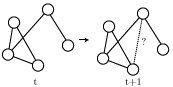
\includegraphics[width=80mm]{img/c2/link_prediction}
 \caption{リンク予測の問題設定}
 \label{c2_link_prediction}
\end{figure}
最初に提唱された論文\cite{liben2007link}では、ソーシャルネットワークの状態が与えられたとき、ユーザ間で交わされる将来の行動を予測する問題として述べられている。この論文では、ノード(ユーザ)間の近さを定義する方法や、全てのエッジ(接続)を通しで見て判断する方法、クラスタリングによる方法などが用いられている。論文で用いられているノード間の近さの定義を図\ref{c2_lp_method}に挙げる(\cite{liben2007link}より引用)。ノード$x$に対し、$x$とつながっているノードの集合を$\Gamma(x)$とする。\par
\begin{table}[tbp]
 \begin{center}
  \begin{tabular}{|l|l|}\hline
  グラフ距離 & (負値にされた) xとyの最短距離 \\ \hline
  共通隣接 & $|\Gamma(x)∩\Gamma(y)|$ \\ \hline
  Jaccard係数 \cite{jaccard1902lois}& $\left| \frac{\Gamma(x)∩\Gamma(y)}{\Gamma(x)∪\Gamma(y)} \right|$ \\ \hline
  Adamic / Adarスコア \cite{adamic2003friends}& $\sum_{z\epsilon \Gamma(x)∩\Gamma(y)} \frac{1}{log|\Gamma(x)|}$ \\ \hline
  優先的選択 & $|\Gamma(x)|・|\Gamma(y)|$ \\ \hline
  \end{tabular}
 \end{center}
 \caption{リンク予測にて、ノード同士の近さを定義する方法}
 \label{c2_lp_method}
\end{table}

リンク予測には様々な応用があり、例えばショッピングサイトのデータ分析に役立てることが出来る\cite{clauset2004finding}。ウェブ工学の問題以外にも応用が可能であり、タンパク質の反応予測(Protein to Protein Interaction, PPI)に用いられたり\cite{bader2003gaining}、テロリストのネットワークや草原の食物連鎖の分析にも役に立っている\cite{clauset2008hierarchical}。全ての部分グラフをカウントする方法はNP困難であり、計算時間的に解くことが難しいことが知られている\cite{gartner2003graph}が、この問題はGraphHopperカーネルを用いることで、現実的な時間で解くことができる\cite{feragen2013scalable}。また、Noisy ORを用いて局所的な情報を統合することにより、効率良く様々な情報を扱わせることができる\cite{changpinyo2013similarity}。
%2011のやつ、flickr, 全解析
%リンク予測の絵
%bag of words?

\subsection{感情分析}
この場合の感情とは、人間が書いた文章から読み取れる感情を指す。ウェブ上の情報収集の自由度が高まるにつれて、ユーザが書いた文章を取得できる機会が増えてきている。その中には、新製品やサービスへの感想やレビューも含まれている。ユーザの属性や行動といった明確な事実だけでなく、他の人がどのような感情を抱いているのかを分析したいという要望が高まり、2000年代に入ってから、人間が書いた文章から人間の感情を読み取るための研究が盛んになった\cite{pang2008opinion}。なお、意見抽出(opinion mining)という語も、多少の差異はあれど、広義には似た内容を指していることが多い。\par
\cite{pang2004sentimental}では、最小カット法を用いることで良い成果が出たとされている。また、\cite{wilson2005recognizing}では、文脈を考慮した単語の感情(positive, negative)を分析して、性能を挙げることに成功している。Google社も、検索エンジンの性能向上のため、感情分析の研究を行っている\cite{godbole2007large}。\par
深層学習との関連で重要な研究として、Stanford大のチームによる文章解析データセットの制作及び、ウェブアプリの開発がある\cite{socher2013recursive}。この研究にて彼らは、感情分析のための大規模なデータセットがそもそも不足しているという問題を解決するため、The Stanford Sentiment Treebankという感情分析のためのデータセットを制作した。さらに、Recursive Neural Tensor Network (RNTN)という深層学習のモデルを構築した。このモデルにより、与えられた文章を構文木に分解した後、各単語が5段階の感情のうちどれにあたるかを分析している。感情は、"very negative"、"negative"、"neutral"、"positive"、"very positive"の5種類に分類される。このモデルは、ソースコードが公開されている他、ウェブページ上にて実際に分析を試してみることができる\footnote{\url{http://nlp.stanford.edu/sentiment/index.html}}。図\ref{c2_rntn_ex}は、論文より引用したもので、文章を実際にこのウェブアプリで分析した様子を表している。赤が強いと悲観的(negative)な言葉、青が強いと好意的(positive)な言葉、というように色分けされている。
\begin{figure}[tbp]
 \centering
  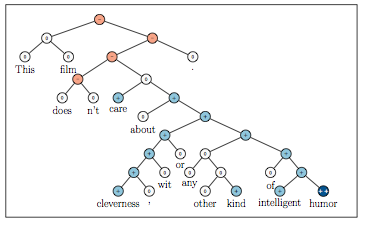
\includegraphics[width=80mm]{img/c2/rntn_ex}
 \caption{Stanford大が製作した、深層学習による感情分析の例}
 \label{c2_rntn_ex}
\end{figure}

\subsection{順位付け学習}
これは、情報検索システムを作る際に用いられる技術である。ユーザが検索をかけるときは、自分が求めた情報だけを、出来るだけ取りこぼし少なく取得したい(適合率と再現率という。\cite{tsujii1999joho})。従来はtf-idfやPageRank\cite{brin1998anatomy}\cite{page1999pagerank}などの単一の指標によって、検索結果を表示させていたが、その後多様なランキング素因を組み合わせるという方法が出現した。どの素因をどのような割合で組み合わせるべきかが問題であり、これに対し機械学習によってランキング関数を作成するアプローチが、順位付け学習である。\par
RankNet\cite{burges2005learning}では、深層構造こそ使っていないが、ニューラルネットワークによってランキング関数の性能をアップさせており、深層学習の応用による性能向上が期待できる。

\section{機械学習で利用される、代表的な分類器}
機械学習のプロセスは、「入力データを、数学的モデルで使える素性に変換する」「素性を数学的モデルに入力して、出力値を得る」「出力を見ながら、モデルを修正する」という行程に大きく分けられる。データの分類問題を機械学習で解く場合、モデルによる出力値が分類結果に対応するよう、モデルを学習させることになる。この場合、モデルのことを分類器とも呼ぶ。\par
機械学習において、素性への変換部分は、データの種類に大きく依存する。一方、分類器に用いる数学的モデルと、モデルの改修法、つまり学習法は、汎用的に使うことができる。あるいは、画像や音声、文章といったデータの多様性を、素性という一般的な数値に落とし込むことで吸収して、汎用的分類モデルでも学習できるようにしている。\par
深層学習、あるいは深層ニューラルネットワーク(多層ニューラルネットワーク)は、汎用的分類モデルの一種である。ここでは、深層学習の他にどのような分類器が存在するのか、代表的なものを述べる。
%\subsection{線形識別モデル}

%\subsection{ロジスティック回帰}
%random forest, ada boost

\subsection{サポートベクターマシン}
サポートベクターマシン(SVM)は、図\ref{c2_svm}のように、データを2つのクラスに分類する能力を持ったモデルである\cite{cortes1995support-vector}。\par
SVMのメインとなる原理は、マージン最大化である。図\ref{c2_svm}は最も単純なSVMの問題を表しており、グラフ上に散らばった黒と白の点を、直線を1本引くことで分けることが目標である。言い換えれば、どの点が黒で、どの点が白なのかを識別する、2クラス分類問題を解こうとしている。緑の線は、分類に失敗している。青の線は分類に成功しているが、後から点線で表された新しい白点が加わると、やはり分類に失敗してしまう。赤の線は、現在見えている点を分類できるだけでなく、新しい点が加わっても正しく識別できる可能性が高い。SVMのマージン最大化とは、各点からの距離(マージン)の和が、最大になるように直線の引き方を決めることである。こうすることにより、汎化性能(訓練時に見えていなかった、新しいデータを正しく分類する性能)が最大になることが知られている。\par
この図のSVMは、データが直線で完全に分類できることを前提にしている。しかし、現実のデータは、\ref{c2_svm_mixed}のように、必ずしも1本の直線にて分類が可能ではない。(3次元以上の場合で言えば、1つの超平面にて分類が可能とは限らない。)このような場合に対応するため、まず非線形関数にてデータを高次元の空間に移し、超平面による分類が出来るように変換する方法が知られている\cite{burges1998tutorial}。ただし、一般に複雑な分類ほど、変換先の次元数が高くなる傾向があり、次元数が増えると、「次元の呪い」と言って、内積計算にかかる時間が指数関数的に増大することがわかっている\cite{bellman1961adaptive}。この計算時間を減少させるため、数式処理によって内積を計算する必要がなくなるように設計された、カーネル関数と呼ばれる変換関数を用いる方法が使われている(カーネルマジック)。
\begin{figure}[tbp]
 \centering
  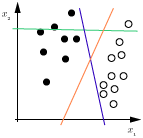
\includegraphics[width=80mm]{img/c2/svm}
 \caption{サポートベクターマシンのマージン最大化}
 \label{c2_svm}
\end{figure}
\begin{figure}[tbp]
 \centering
  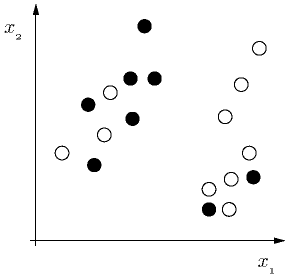
\includegraphics[width=80mm]{img/c2/svm_mixed}
 \caption{直線にて分類できない場合}
 \label{c2_svm_mixed}
\end{figure}
SVMは、広くその信頼性が認められたモデルの1つであり、ライブラリの利用方法も確立している。例えば、LIBSVM\footnote{\url{http://www.csie.ntu.edu.tw/~cjlin/LIBSVM/}}やLIBLINEAR\footnote{\url{http://www.csie.ntu.edu.tw/~cjlin/LIBLINEAR/}}は使用が容易なライブラリとしてよく知られている。これらのライブラリを使うと、簡単な所定の方式に沿って入力データファイルを用意し、CUI上で2,3回の操作をするだけで、SVMによる分類を行わせることができる。このとき、利用者が自分でプログラムを書く必要は全くない。プログラムを書かないで済むと、手軽に利用することができ、またバグを起こす危険性が非常に少なく安全に使うことができる。\par
深層学習については、このようなライブラリはまだ存在していないため、深層学習の代表的なアルゴリズムについて、プログラム無しで利用できるようなライブラリの整備が望まれる。
\subsection{ニューラルネットワーク}
ニューラルネットワークは、人間の脳の構造を模倣した数学的モデルである。人間の脳は、ニューロンと呼ばれる神経細胞が大量に接続されて出来ている。ニューロンが電気信号を伝達することで、様々な脳の働きが行われている、と考えられている。プログラム上で表現されるニューラルネットワークには、人間の脳の動作との相違点もあり、脳が行っている計算を正しくシミュレートしているとは言い難い面もある\cite{kawato1998}が、機械学習のモデルとしては広く使われてきた。\par
\subsubsection{ニューラルネットワークの伝達方式}
以後、機械学習におけるニューラルネットワークのニューロンを、慣例に従ってユニットと呼ぶことにする。ニューラルネットワークでは、ユニットからユニットへの接続が網目のように広がっている。ユニットは入出力の機能を持つ。これは、生体におけるニューロンが、他のニューロンから化学的な刺激を受け取り、受け取った刺激に応じて自らも他のニューロンを刺激する構造を真似ている。ユニットは入力を受け取ると、活性化関数(activation function)を使って入力値を変換し、接続先のユニットへ出力する。このとき、ユニットからユニットへの結線に、重み(weight)と呼ばれる係数を付与して、出力を変化させることが普通である。これは、生体のニューロン同士の接続が、脳の学習につれて強固になり、刺激がより伝わりやすくなっていくことに対応させている。
\subsubsection{パーセプトロン}
パーセプトロン(perceptron)とは、ニューラルネットワークの一種である。複数のユニットをまとめたレイヤーが、いくつか重なって出来ており、値の伝達は入力レイヤーから出力レイヤーへの一方向に限られているものを指す(前送り)。狭義には、単層かつ活性化関数にヘビサイド関数を用いた2クラス分類モデルのみを指すこともある。\par
始めに提唱されたのも、入力層と出力層の2層から成る、単層パーセプトロンと呼ばれるモデルだった\cite{rosenblatt1958perceptron}。このモデルは、後に線形関数しか近似できないことがわかり、いったん下火になった\cite{minsky1988perceptrons:}。例えば、単層パーセプトロンでは、非線形関数であるXOR関数を学習させることが出来なかった。\par
しかし、隠れ層を追加し、活性化関数にシグモイド関数などの非線形関数を用い、さらにバックプロパゲーションという方法で学習を行わせることにより、非線形関数を近似可能となることがわかり、再び有用な識別モデルとして脚光を浴びた\cite{rumelhart1986learning}\cite{funahashi1989on-the-approximate}。これを単層パーセプトロンと区別して、多層パーセプトロン(Multi Layer Perceptron, 以下MLP)とも呼ぶ。このモデルは単純な2クラス分類モデルの範囲を逸脱しており、元々のパーセプトロンとはやや異なるものだが、慣例的にこのように呼ばれている。\par
バックプロパゲーションは教師有り学習の一種である。出力層におけるモデルが出した推定値と、教師データの結果が異なっている場合、教師データからの推定誤差(error)が減少するように、モデルのパラメータを修正する。MLPの場合、モデルのパラメータとはユニット間の伝達にかかる重み係数のことである。パラメータの修正値の仕方にはバリエーションがあるが、最もよく使われるのは確率的勾配降下法(以下SGD)と呼ばれる方法である。これは確率変数に拡張された一種の再急降下法である。直感的に言えば、微分によって、その場で推定誤差が最も急速に減少するパラメータの修正方向を算出し、その方向に向かってパラメータを変化させる。SGDを少し変化させ、複数のデータによる誤差を一度に処理するバッチ勾配降下法(BGD)や、SGDの1次精度に対し、2次精度までの情報を使う共役勾配法(Conjugate Gradient Method, CG)も存在する。\par
%vanishing error problem
バックプロパゲーションを行うためには、活性化関数が微分できることが重要である。シグモイド関数は、元々使われていたヘビサイド関数に形が似ている上に、微分が容易という点でバックプロパゲーションとの親和性が高く、有利である。しかし、シグモイド関数のデメリットとして、入力と重みの積が大きくなるにつれて、誤差への反応が小さくなってしまい、学習の進行が遅くなるという問題を抱えていた。この問題は、特にバックプロパゲーションで伝播する距離が長くなる構造にて顕著になった\cite{hochreiter1998the-vanishing}\cite{hochreiter1998the-vanishing}。このため、多層ニューラルネットワークを学習させる方法は長い間課題となっていた。